%!TEX root = research_proposal.tex

\pagenumbering{arabic}
\setcounter{page}{1}

\chapter{Introduction}

Maintenance activities are known to be costly and challenging \cite{Pressman2005}. Studies have shown that the cost of software maintenance can reach up to 70\% of the overall cost of the software development process \cite{HealthSocial2002}.

Lehman's laws of software evolution apply to three different types of software $S$, $P$ and $E$ \cite{lehman1980programs}. S-Software are written according to an exact specification of what that program can do, E-program are is written to perform some real-world activity; how it should behave is strongly linked to the environment in which it runs, and such a program needs to adapt to varying requirements and circumstances in that environment and, finally, P-software are program is written to implement certain procedures that completely determine what the program can do.

\begin{itemize}
	\item ``Continuing Change'' — an E-type system must be continually adapted or it becomes progressively less satisfactory
	\item ``Increasing Complexity'' — as an E-type system evolves, its complexity increases unless work is done to maintain or reduce it
	\item  ``Self Regulation'' — E-type system evolution processes are self-regulating with the distribution of product and process measures close to normal
	\item ``Conservation of Organisational Stability (invariant work rate)'' - the average effective global activity rate in an evolving E-type system is invariant over the product's lifetime
	\item ``Conservation of Familiarity'' — as an E-type system evolves, all associated with it, developers, sales personnel and users, for example, must maintain mastery of its content and behavior to achieve satisfactory evolution. Excessive growth diminishes that mastery. Hence the average incremental growth remains invariant as the system evolves.
	\item ``Continuing Growth'' — the functional content of an E-type system must be continually increased to maintain user satisfaction over its lifetime
	\item ``Declining Quality'' — the quality of an E-type system will appear to be declining unless it is rigorously maintained and adapted to operational environment changes
	\item ``Feedback System'' — E-type evolution processes constitute multi-level, multi-loop, multi-agent feedback systems and must be treated as such to achieve significant improvement over any reasonable base
\end{itemize}

On a lighter note, Brian Russell resumed this into what he -- ironically -- named the Laws of Software Relativity:

\begin{itemize}
\item As a software project approaches release, its mass increases.
\item The energy required to release a software project is inversely proportional to the time before a scheduled release.
\item It takes infinite energy to release a finished product on time; therefore, all software projects are both incomplete and late.
\item Time is relative to the observer of a software project. The last month of development appears to an outside observer to take a year.
\item If a software project becomes too large, it will collapse into a black hole. Time and money are absorbed but nothing ever comes out.
\end{itemize}

While these laws, written from 1974 to 1996, still very much apply to nowadays software engineering, engineers and practitioners have created tools, technics and processes to control their negative impacts.
For instance, most of real world project's -- in opposition to test / very small size projects -- host their source code on a version control system \cite{rochkind1975source} that is able is able to keep track of the different revisions of a system and of the different changes made by the developers of the team.
Version control systems help to control the {\it continuing change}, {\it increasing complexity} and {\it continuing growth} rules' effects.
In order to manage the {\it feedback systems} and {\it declining quality} rules, organization use issue \& project tracking system to assign tasks to developers, report unexpected behaviors or crashes and track advancement.

In the last decade, source code revision control system and issue \& tracking system have grown to contain hundreds of thousands of revision, issues and tasks per project.
Naturally, this plethora of data pushed researchers across the world to conduct hundreds of studies in several active research fields: Bug reproduction, bug triaging, duplicated bug identification, bug comprehension, bug re-production.

Mining system and issue \& tracking and source code version control systems is perhaps one of the most active research fields today. The reason is that their analysis provides useful insight that can help with many maintenance activities such as bug fixing \cite{Weiss2007,Saha2014}, bug reproduction \cite{Artzi2008,Jin2012,Chen2013}, fault analysis \cite{Jiang2012,Jin2013}, etc. This increase of attention can be further justified by the emergence of many open source bug tracking systems, allowing open source software teams to make their bug reports available online to researchers.

\section{Preliminaries\label{sec:preliminaries}}


In this section, we explain what are version control systems (in \ref{sec:version-control}) and Issue \& project tracking system (in \ref{sec:issue-tracking}). If one were to be familiar with Svn\footnote{https://subversion.apache.org/}, Git\footnote{https://git-scm.com/}, Mercurial\footnote{https://mercurial.selenic.com/}, Bugzilla\footnote{https://www.bugzilla.org/}, Jira\footnote{https://www.atlassian.com/software/jira} and Github\footnote{https://github.com/}, one can skip to section \ref{sec:outline}.

\subsection{Version control systems\label{sec:version-control}}

Version control consist in maintaining the versions of files -- such as source code and other software artifacts.
This activity is extremely complex and cannot be done by hand on real world project\footnote{Once again, real world project qualify projects that done in an industrial environment rather than school or so.}.
Consequently, numerous software have been created to help practitioners to manage the version of their software artifacts.
Each evolution of a software is a version\footnote{Software version is not to be confused with the version of a software which refer to the shipping of a final product to customers.} (or revision) and each version (revision) is linked to the one before through modifications of software artifacts.
These modifications, that consist in updating, adding or deleting software artifacts, can be referred as \texttt{diff}, {\tt patch} or {\tt commit}
\footnote{These names are not to be used interchangeably as difference exist.}.
Each \texttt{diff}, {\tt patch} or {\tt commit} own the following characteristics:

\begin{itemize}
\item Number of Files: The number of software artifacts that have been modified, added or deleted.
\item Number of Hunks: The number of consecutive block of modified, added or deleted lines in textual files. Hunks are useful to determine, in each file, how many different places the developer have modified.
\item Number of Churns:  The number of lines modified. However, the churn value for a line change should be at least two as the line had to be deleted first and then added back with the modification.
\end{itemize}

\subsubsection{Providers\label{sec:revision-provider}}

In this document, we will mainly refer to three version control systems: {\tt Svn}, {\tt Git} and, in a lesser extent, {\tt Mercurial}. {\tt SVN} is distributed by the Apache foundation and is a centralized concurrent version system that can handle conflict in the different versions of different developers and it is widely use.
At the opposite, {\tt Git} is a distributed revision control system -- originally developed by Linus Torvald -- where revisions can be kept locally for a while and then shared with the rest of the team.
Finally {\tt Mercurial} is also a distributed revision system but share a lot of concepts with {\tt Svn}.
Consequently, it will be easier for folks used to {\tt Svn} to switch to a distributed revision system if they use {\tt Mercurial}.

\subsection{Issue \& Project Tracking Systems\label{sec:issue-tracking}}

Issue \& project tracking systems allow end-users to directly create bug reports (BRs) to report on system crashes and manager can create tasks to drive the evolution forward.
These systems are also used by development teams to manage the BRs, and keep track of the fixes.

The life cycle of an issue is as follows: After an issue is submitted by an end-user, it is set to the {\tt UNCONFIRMED} state until it receives enough votes or that a user with the proper permissions modifies its status to {\tt NEW}.
The bug is then assigned to a developer to fix it.
When the bug is in the {\tt ASSIGNED} state, the assigned developer(s) start working on the issue.
A fixed issue moves to the {\tt RESOLVED} state. Developers have five different possibilities to resolve an issue: {\tt FIXED}, {\tt DUPLICATE}, {\tt WONTFIX}, {\tt WORKSFORME} and {\tt INVALID}.

\begin{itemize}
	\item {\tt RESOLVED/FIXED}: A modification to the source code have been pushed, i.e., a changeset (also called patch) has been committed to the source code management system and fixes the issue.
	\item {\tt RESOLVED/DUPLICATE}: A previously submitted issue is being processed. The bug is marked as duplicate of the original bug.
	\item {\tt RESOLVED/WONTFIX}: This is applied in the case where developers decide that a given bug will not be fixed.
	\item {\tt RESOLVED/WORKSFORME}: If the issue cannot be reproduced on the reported OS / hardware.
	\item {\tt RESOLVED/INVALID}: If the issue is not related to the software itself.
\end{itemize}

Finally, the issue is {\tt CLOSED} after it is resolved.
An issue can be reopened (set to the {\tt REOPENED} state) and then assigned again if the initial fix was not adequate (the fix did not resolve the problem). The elapsed time between the issue marked as new one and the resolved status is known as the {\it fixing time}, usually in days.
If the issue is reopened then the days between the time the issue is reopened and the time it is marked again as {\tt RESOLVED/FIXED} are cumulated. Issues can be reopened many times.

Tasks follow a similar life cycle at the exception of the {\tt UNCONFIRMED} and {\tt RESOLVED} states.
Tasks are created by management and do not need to be confirmed in order to be {\tt OPEN} and {\tt ASSIGNED} to developers.
When a task is complete, it will not go to the {\tt RESOLVED} state but to the {\tt IMPLEMENTED} state.
Issue are considered as problem to eradicate in the program and thus, fold into the maintenance activity.
Tasks are considered as new features or amelioration to include in the program and fold into the evolution activity.

Issue and tasks can (and must according to \cite{Bettenburg2008}) have a
severity. The severity is a classification of a issue to indicate the
degree of negative impact on the quality of software and can
evolve at any point during the lifecycle of the bug. The possible severities are blocker (blocks
development and/or testing work) critical (crashes, loss of
data, severe memory leak), major (major loss of function),
normal (regular issue, some loss of functionality under
specific circumstances), minor (minor loss of function, or
other problem where easy workaround is present) trivial
(cosmetic problem like misspelled words or misaligned text).


The relationship between an issue or task and the actual modification can be hard to establish and it has been a subject for various research studies (e.g., \cite{Antoniol2002,Bachmann2010,Wu2011}) for the simple reason that they are in two different systems: the revision and the issue management systems. While it is considered a good practice to link each issue with the source code revision system by indicating the issue $\#id$ on the modification message, more than half of the issues are not linked to a modification.


\subsubsection{Providers\label{sec:bug-provider}}

 In this study, we collect data from four different bug tracking systems: $Bugzilla$, $Jira$, $Github$ and $Sourceforge$. $Bugzilla$ belongs to the Mozilla foundation and have first been released in 1998. $Jira$ is provided by Altassian have been released 13 years ago, in 2002. $Bugzilla$ is 100\% open source and its difficult to estimate how many project use it.
 However, we can, without any risks envision that they have a great share of the market as major organization such as Mozilla, Eclise and the Apache Software Foundation use it.
 $Jira$, in the other hand, is a commercial software -- with a freemium buisiness model -- and Altassian claims that they have 25,000 customers over the world.

 $Github$ and $Sourceforge$ are different from $Bugzilla$ and $Jira$ in a sense that they were created as revision system and evolve, latter on, to add Issue and project management capabilities to their softwares. Nevertheless, this common particularity have the advantage to ease the link between issues and source code.



\section{Motivation}

Architects, the ones that design buildings -- where mistakes cost lives -- spend at least five years at school and possibly their whole carriers to study, understand and reproduce great designs made by great architects.
Software architects, however, begin in programing 101 by displaying the famous ``{\tt Hello World}'' statement and exponentially increase the complexity of their programs over their years of study and work.
At some point, they will earn the title of software architect (or technical leader) because they have designed, maintained and evolved {\it enough} programs to be trustworthy on the matter.
However, unlike building architects they have to learn how to recognize, analyze and reproduce great architectural choices by themselves on the in addition of their day to day work.
Of couse, software developers do learn good practices such as Design Patterns \cite{Gamma2008} but in a very few occasions they will be presented with a state-of-the-art programs built by great developers (Amy Brown {\it et al.} propose exactly that in their books \cite{chansler2011architecture, AmyBrown2012,Armstrong2013}).

While this research is not about reforming how programming classes are thaught, we still want to ease the access to this knowledge for developers during their programming sessions in order to ship better programs.

In this research proposal, we shift the focus from merely mining revision and issue management system, where knowledge of great developers lies, to integrate them at their rightful place: as the keystone of software development and evolution activities.
Extracting ground truth from repositories helped engineers and practitioners to be better at building softwares as they know, for example,{\it how long it will take to fix a bug} \cite{Weiss2007}, {\it what's make a good bug report} \cite{Bettenburg2008} or {\it how to fix long-lived bugs} \cite{Saha2014}.
Using these discoveries, tools can be created, in a per organization basis, to fit particular requirements such as programming language, development processes or particular threshold. If we want to truthfully and deeply modify the software engineering landscape to have better softwares in terms of quality, maintainability and evolvability we need to provide these information during the development, maintenance and evolution processes according to a specific context in an easy, reliable, free way.

If we look back at the history of software engineering, the increase of processors' speed allowed one to have a compiler on its own machine rather than sending one's code to the mainframe and receive compilation errors hours (days) later. This allowed, among other factors, the democratization of software engineering as {\it everyone}, belonging to a major organization or not, became able to build code. We believe that, it is now time to allow developers, engineering and practitioners, regardless of their programming language and contextual environment not only to write and build code but to write and built qualitative, robust, resilient, easy to maintain and to fix code. What better way to do so than to {\it stand on the shoulder of giants} by having access to the whole open sources repositories, including but not limited to, issues, tasks, bug fixes, patches, comments, good practices break down to the right level and provided at the right time during day to day programming sessions ?

What we concretely propose is an open-source, free, automatable tool suite that will allow everyone to (1) automatically reproduce field crashed in a controlled lab environment without any privacy concerns, (2) search in natural language the issues, comments, bugs, patches and fixes of tens of thousands of open source project, (3) prevent the insertion of defects in the source code during programming sessions by providing examples of the similar defect and how it has been fixed with a programming language abstraction. To support these tools we propose an empirical bug taxonomy (4).

\section{Thesis Contributions}


In this section we present the problems in the literature (Section \ref{sec:pb-litterature}), the research challenges we face in our work (Section \ref{sec:challenges}). Sections \ref{sec:scope} and \ref{sec:objective-thesis} present the scope and the contributions of this research.

\subsection{Problems in the Literature\label{sec:pb-litterature}}

\begin{itemize}
	\item {\bf Problem 1} : As shown by Figure \ref{fig:scholar}, the proportion of empirical studies and studies based on mining software repositories regarding to software quality is increasing exponentially since 2010 (\cite{Kim2011a,Lee2011a,Sun2011,Bhattacharya2011,Tian2012a,Zimmermann2012, Shang2013,Chen2014,Mcintosh,Hemmati2015} are some noticeable examples).
	Yet, all this accumulated knowledge fail to be useful in day-to-day programming session and to effectively improve the overall quality of software produced nowadays.

	\begin{figure}[h!]
	  \centering
	  	    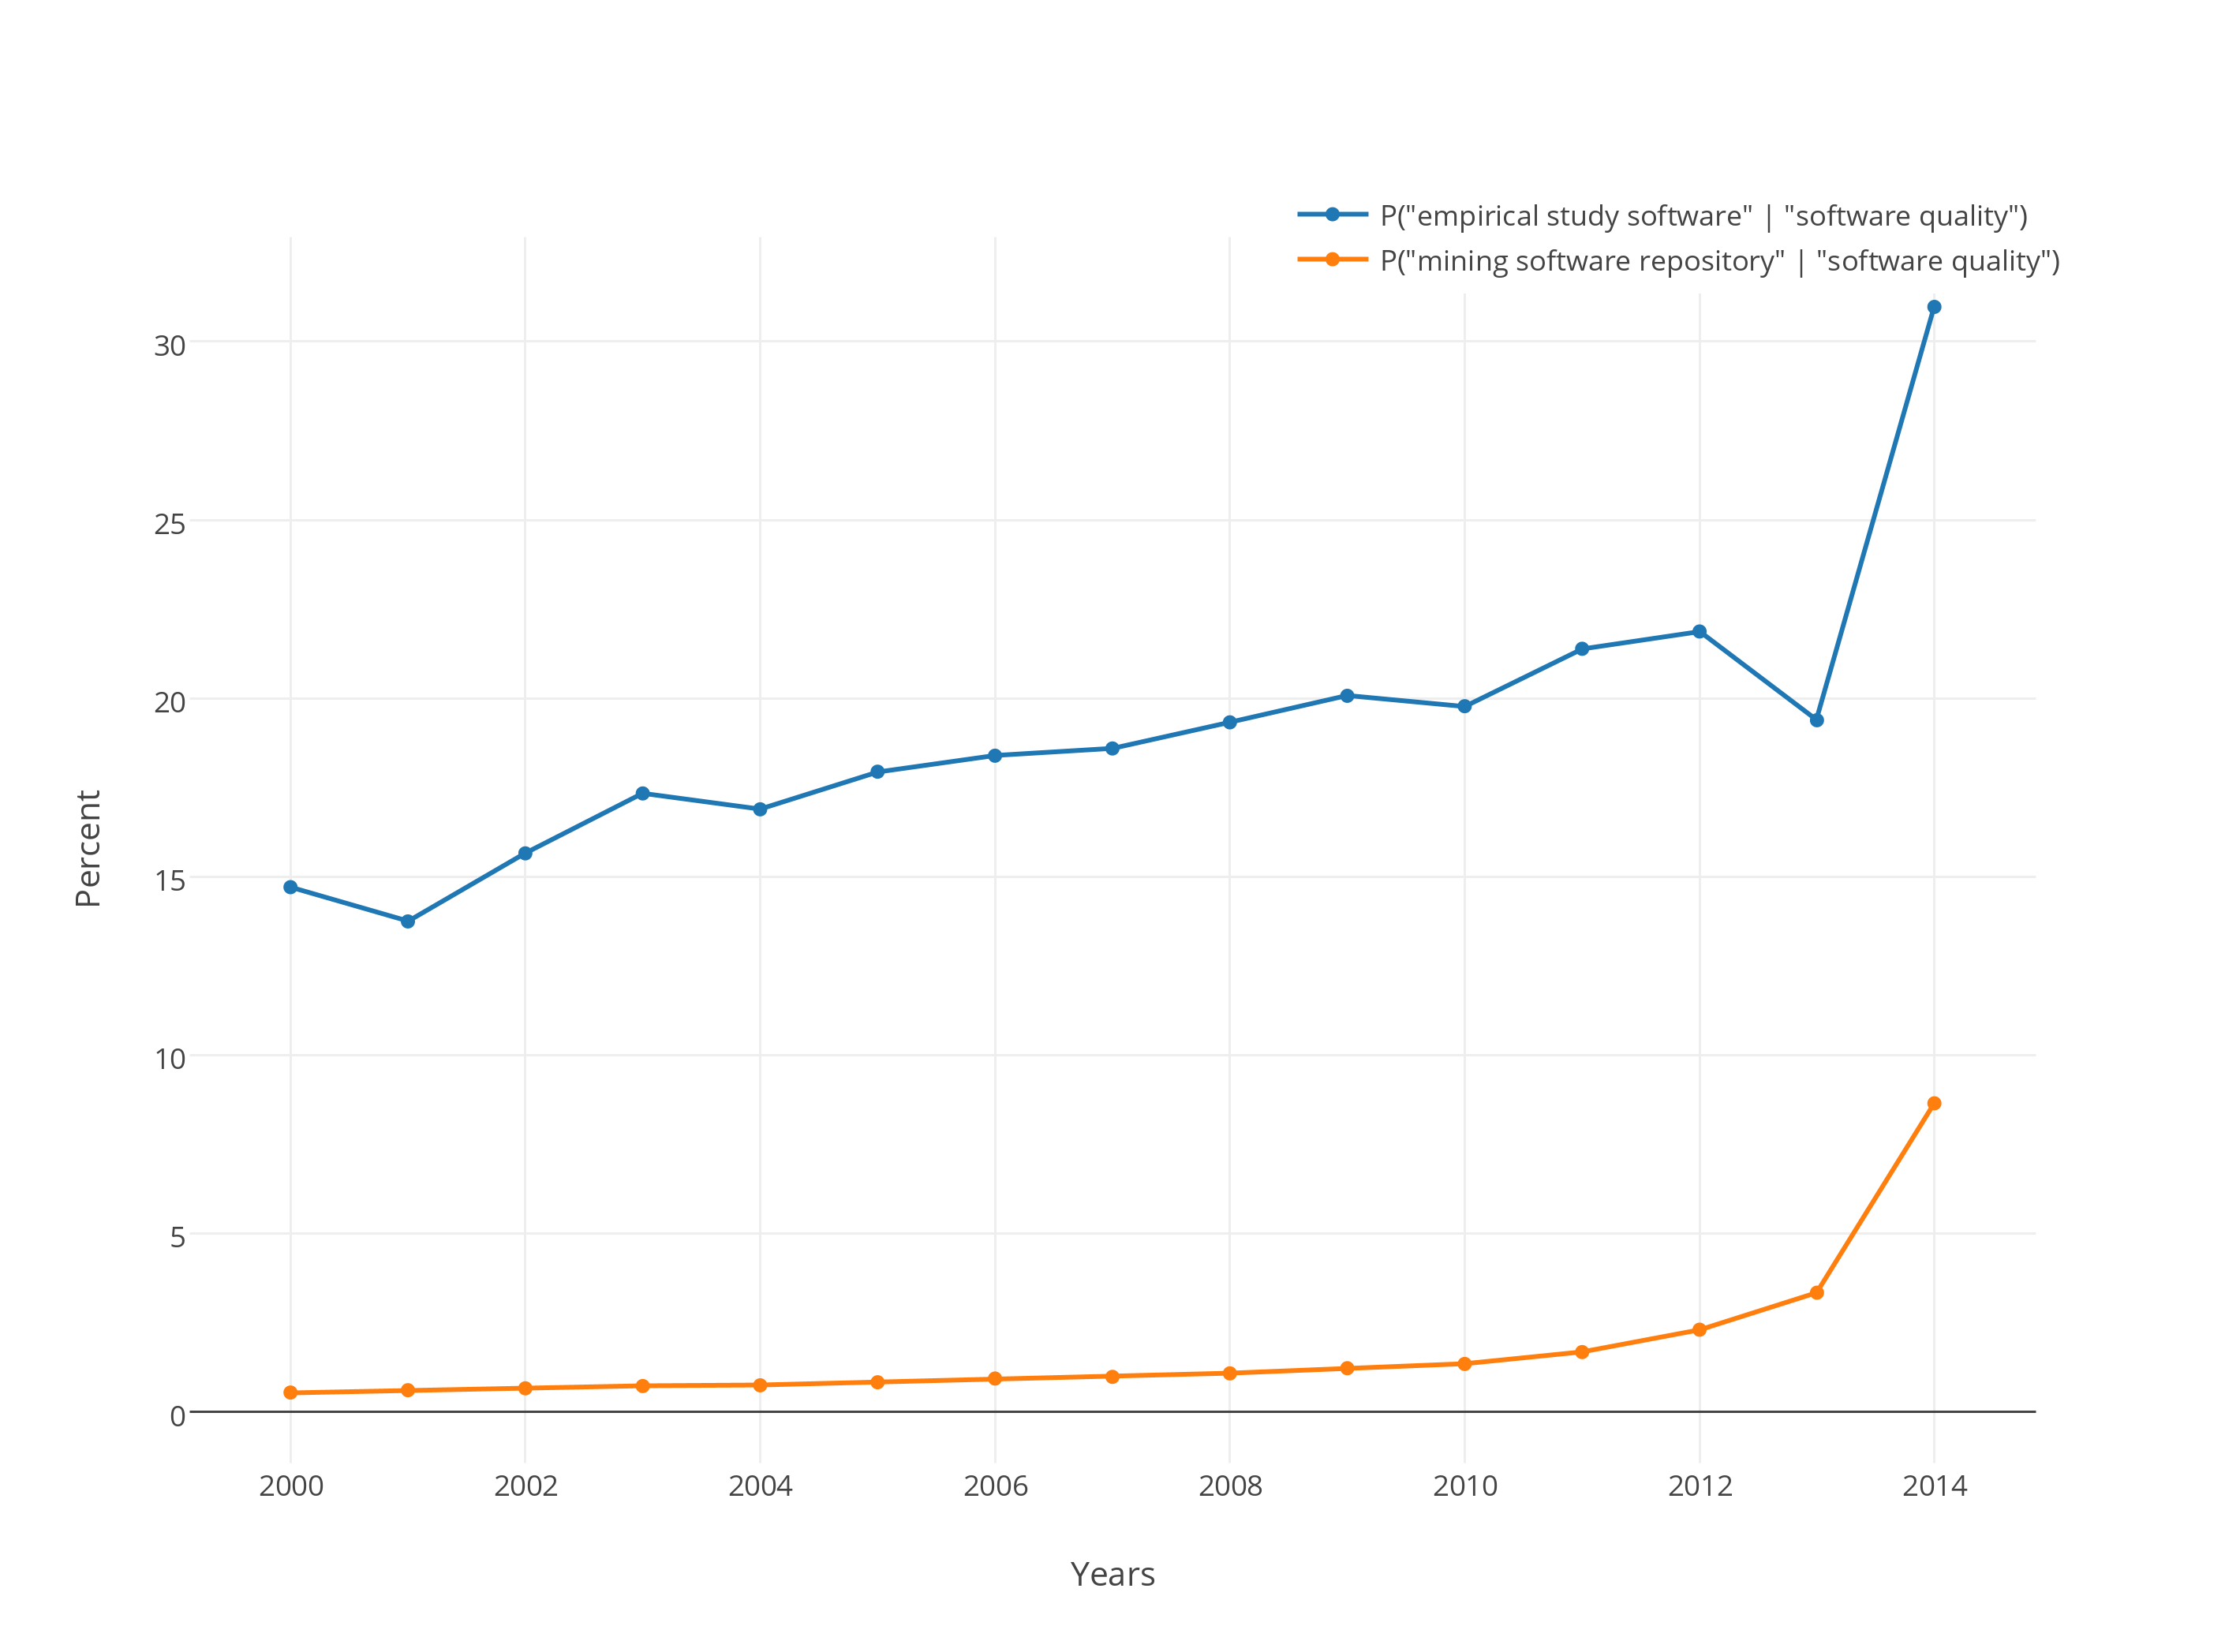
\includegraphics[scale=0.7]{media/scholar.png}
	    \caption{Proportion of papers containing ``Empirical Study'' or ``Mining software repository'' with regards to the paper in Software quality indexed by Google Scholar	\label{fig:scholar}}
	\end{figure}

	\item {\bf Problem 2} : The literature contains numerous paper about tools that improve the overall software quality with static \cite{Dangel2000, burn2003checkstyle,Hovemeyer2007,Moha2010} and dynamic \cite{Nayrolles,Nayrolles2013a,Palma2013} analysis. To the best of our knowledge approaches leveraging other sources to improve quality or efficiency mostly rely on web-search \cite{Brandt2009,Rahman2013,Montandon2013}.

	\item {\bf Problem 3} : There is no approach that support the natural language search and comparison of issues, source code and tasks regardless of the project, repository, revision and issue management system and programming language. Such an approach could dramatically transform software engineering processes. Moreover, the data contained in these repositories lack a taxonomy, as for clone detection \cite{CoryKapser}, to classify the research.
\end{itemize}

\subsection{Research Challenges\label{sec:challenges}}

\begin{itemize}
	\item {\bf Challenge 1} : Issues \& projects and revision systems are plenty and they all have specific processes and limitations. Mining them all in order to have a representative model is challenging. Despite the parsing aspect, gigabytes of new data are generated every day thus, storing accessing to these data in reasonable time will require innovations in high density nosql databases \cite{Nayrolles2014b} and web servers \cite{Nayrolles2013b,Nayrolles2014c}. Moreover, creating the relationship between both systems is still an open issue as discussed in sections \ref{sec:issue-tracking} and \ref{rel:issue-rela}.

	\item {\bf Challenge 2} : Providing code samples break down to the right level, at the right time in order to solve a problem  or improve the current code in terms of quality, performances or reliability during a programming session will force us to improve current approaches of source code transformation and normalization \cite{Cordy2006a, Cordy2006,Roy2008,Cordy2011}.
\end{itemize}

\subsection{Scope of the research \label{sec:scope}}

The area of this research is to improve the processes of software engineering by providing contextual informations, in order to improve the quality, the performance, the reliability of a given code during a programming session. These contextual informations will come from mining issue \& project and revision systems. Hence, we will not define what are the good or bad practices to improve the quality, the performance, the reliability of a given code but rely on the mined data.

\subsection{Thesis contributions\label{sec:objective-thesis}}

Figure \ref{fig:proposal} depicts our proposed solution for fulfilling the objectives we presented in section \ref{sec:objective-thesis}.
First of all, a end-user (team member) will report an issue (open a task) in one the organization issues \& project management system. This can be done in $Sourceforge$, $Bugzilla$, $JIRA$ or $Github$ which are the system we want to support first as described in section \ref{sec:bug-provider}.

\begin{figure}[h!]
	\centering
	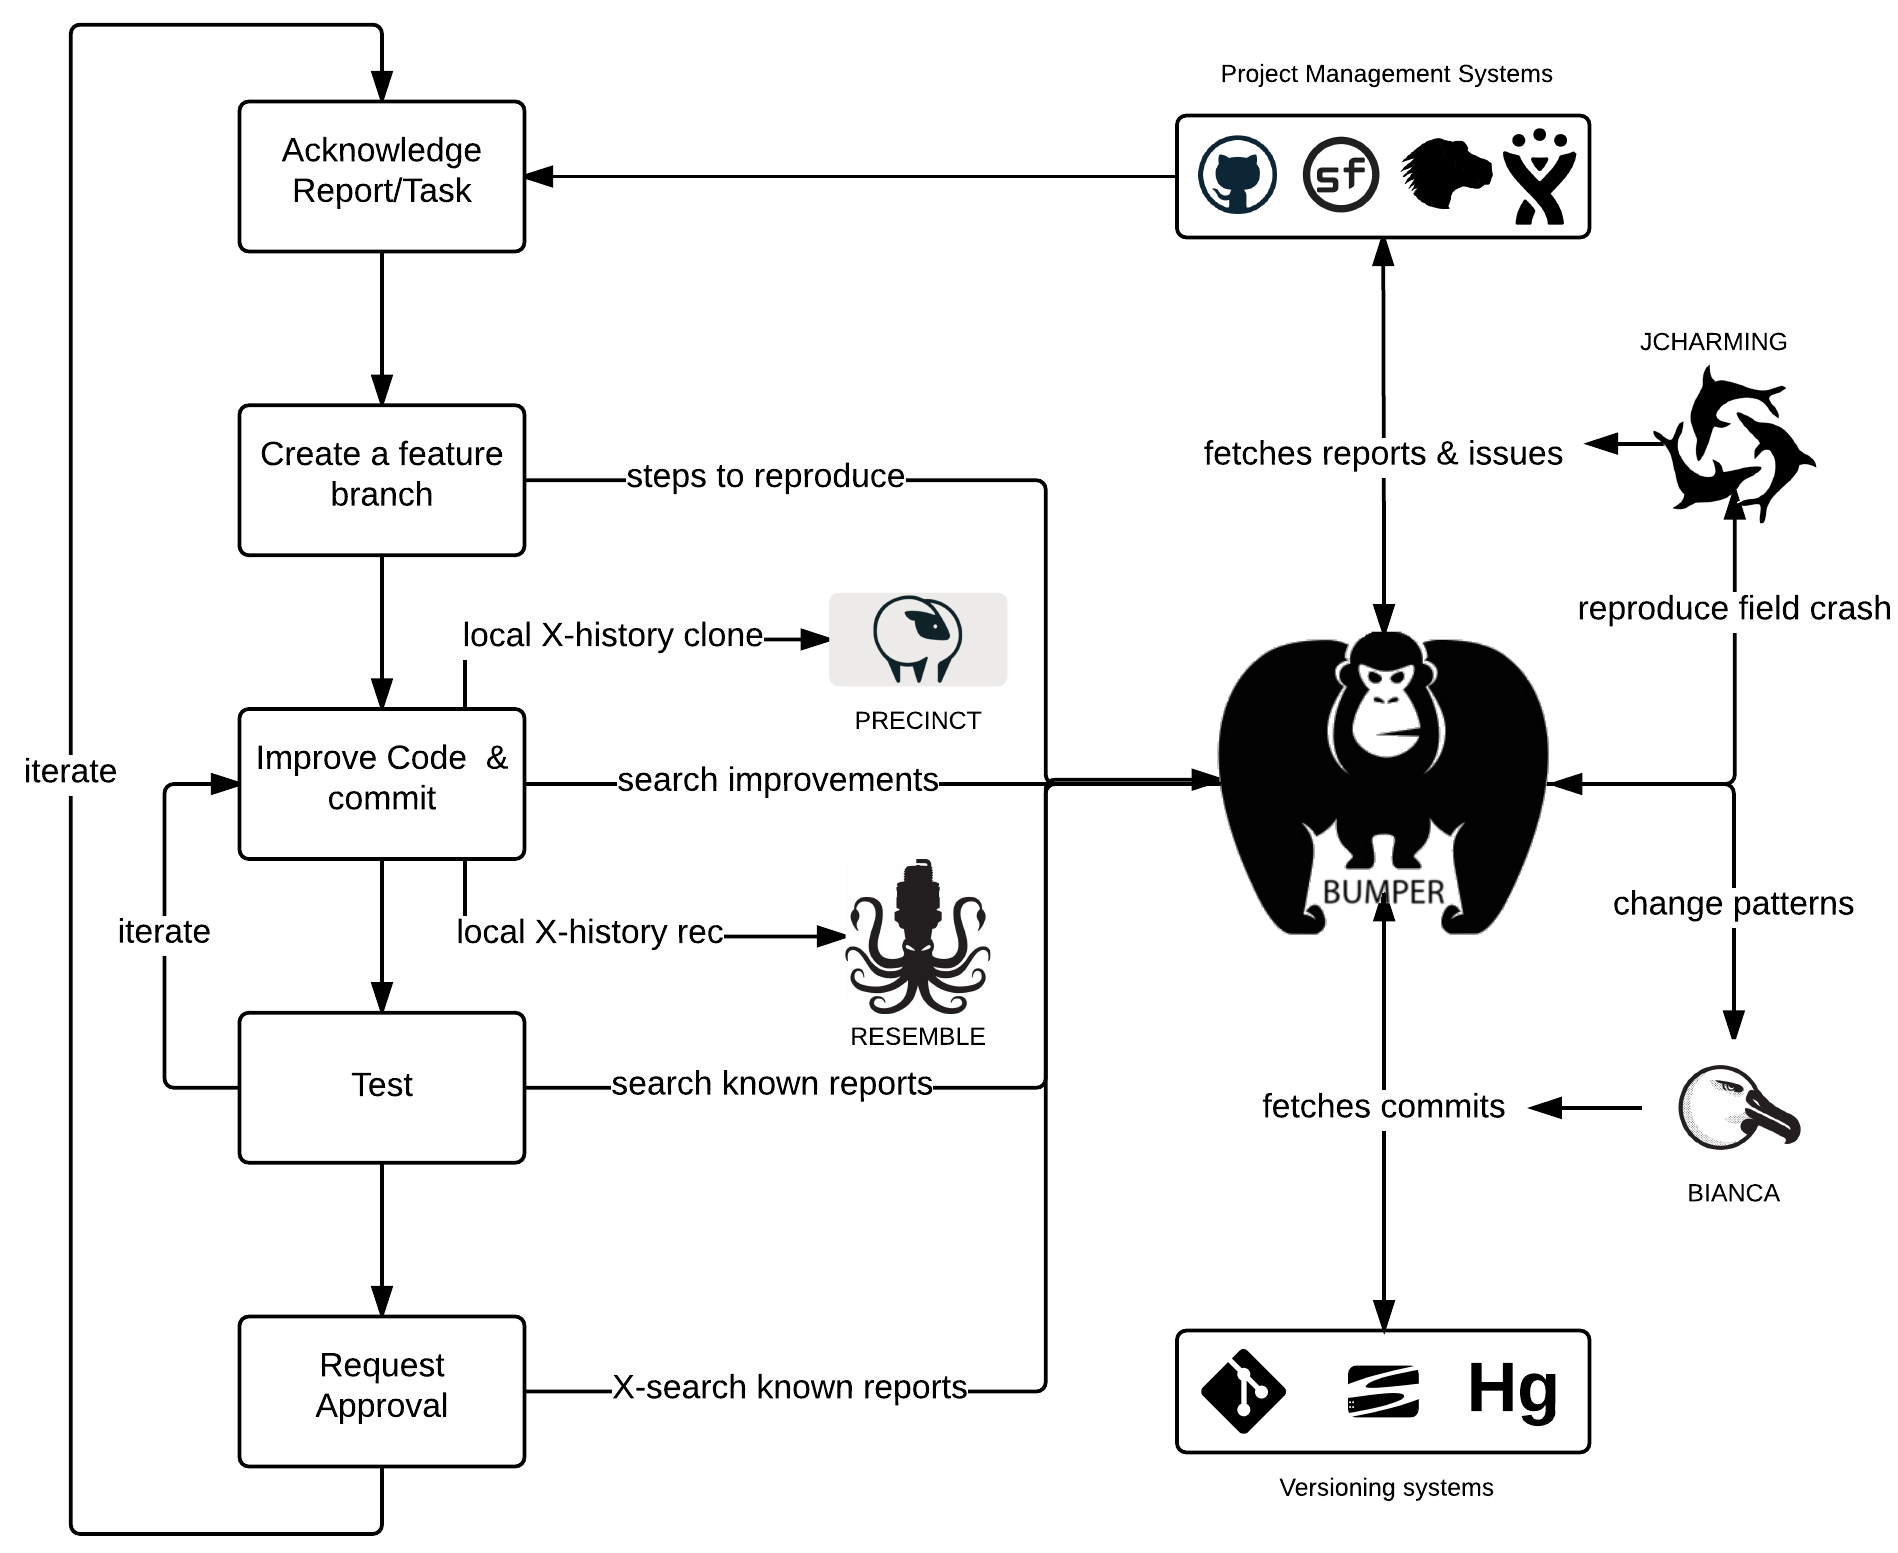
\includegraphics[scale=0.9]{media/proposal.png}
	\caption{Proposed Architecture}
	\label{fig:proposal}
\end{figure}


Issues (tasks) are  mapped with their fixes (implementations) inside {\tt BUMPER} (BUg MetarePository for dEvelopers and Researchers). The source code is fetched from the supported version system: $Git$, $Svn$, $Mercurial$ presented in section \ref{sec:version-control}.
{\tt BUMPER} is a meta-repository that make issues, tasks and related source code searchable using natural language  (in opposition to structured query language).
When an issue is reported, {\tt JCHARMING} (Java CrasH Automatic Reproduction by directed Model checkING) will fetch the content of the issue and try to create a scenario to reproduce the on-field crash. In case of success, the developer assigned to this issue will be notified and the scenario stored in {\tt BUMPER}.
The developer assigned to the task or the issue will modify the code and, in real time, very much like intellisense or auto-completion in modern IDE, {\tt RESEMBLE} (REcommendation System based on cochangE Mining at Block LEvel) will propose improvements or follow up on the developer's code using the decades of history of {\tt BUMPER}. Once s/he is done, s/he submit a commit, patch or diff to the version system.
However, before s/he allowed to do so, {\tt BIANCA} (Bug Insertion ANticipation by Clone Analysis at commit time) will kicks in and query {\tt BUMPER} looking for similar modifications in other projects and even other programming languages that led to the insertion of a defect in order to warn the user about potential hazardous code.


The bug taxonomy required to build {\tt BUMPER}, {\tt BUMPER} itself, {\tt JCHARMING}, {\tt RESSEMBLE} and {\tt BIANCA} are presented in sections \ref{sec:taxo}, \ref{sec:BUMPER}, \ref{sec:JCHARMING}, \ref{sec:RESEMBLE} and \ref{sec:BIANCA}, respectively. In addition, we list parts that have been published in peer-reviewed conferences in section \ref{sec:current-state} and our publication plan in \ref{sec:publication-plan}.

As a motivating example, we draft the following scenario. Table \ref{tab:bumper-hypo} presents hypothetical data stored in {\tt BUMPER} in terms of sequence \#id, sequence of code blocks, a flag to known if a said sequence introduced an issue in a given system and step to reproduce the issue if any.

\begin{table}[h!]
\centering
\begin{tabular}{c|c|c|c|c}
Seq \#ID & Language \#ID & Blocks & Root of Issue & Steps to reproduce \\ \hline \hline
1        & 1             & A-A-B-C-A-A   & Yes  & E-F-G         \\
2        & 1             & A-A-B-C       & No   & -         \\
3        & 2             & D-E-A-C       & No &  - \\ \hline \hline
\end{tabular}
\caption{Hypothetical {\tt BUMPER} data}
\label{tab:bumper-hypo}
\end{table}

During a programming session, let's assume that a developer have blocks $A-B-C$, then {\tt RESEMBLE} will recommends to transform the current code to $A-A-B-C$ as it seams to be the right thing to do.
If the developer follows {\tt RESEMBLE} recommendation and then adds another two $A$s and commit his/her changes.
The sequence is now $A-A-B-C-A-A$ and {\tt BIANCA} will raise a warning saying that this sequence is known to be the root of an issue and invite the developer to execute the steps $E-F-G$ -- that were produced by {\tt JCHARMING} -- in order to see if s/he did introduce a defect. Moreover, {\tt BIANCA} will take the time to compare $A-A-B-C-A-A$ and $D-E-A-C$ using our normalization algorithms even if they are not in the same programming language.
Finally, when a new issue is submitted, {\tt BUMPER} indexes it and {\tt JCHARMING} tries to reproduce it and update the step to reproduce part of {\tt BUMPER}.

We can envision the potential of such a system and the its complexity knowing that it would contain millions of issues, hundreds of thousands projects, dozens of programming languages and will help developers leveraging the knowledge of other developers.

To summarize this thesis have four main contributions:

\begin{itemize}
	\item To provide a taxonomy of software issues to classify the research.
	\item To propose approaches to aggregate as many issues and revisions systems as possible.
	\item To propose approaches to reproduce field crashes in lab environment using the issue content.
	\item To propose a context-aware IDE that will improve day-to-day programming session with concise and appropriate code samples.
\end{itemize}



\section{Outline\label{sec:outline}}

The remainder of this proposal is organized as follows. The following section discuss the problems we propose to solve and their motivations. Chapter \ref{chap:relwork} summarizes the related work.
Chapter \ref{chap:methodology} introduces the proposed approach, the framework, and the preliminary experiments along with the results.
Chapter \ref{chap:plan} presents the current state of the research, and highlights our key current contributions and future research directions along with with a possible publication schedule.
Finally, Chapter \ref{chap:conclusion} provide some concluding remarks and future works.
